%-----------------------------------LICENSE------------------------------------%
%   This file is part of tikz_figures.                                         %
%                                                                              %
%   tikz_figures is free software: you can redistribute it and/or              %
%   modify it it under the terms of the GNU General Public License as          %
%   published by the Free Software Foundation, either version 3 of the         %
%   License, or (at your option) any later version.                            %
%                                                                              %
%   tikz_figures is distributed in the hope that it will be useful,            %
%   but WITHOUT ANY WARRANTY; without even the implied warranty of             %
%   MERCHANTABILITY or FITNESS FOR A PARTICULAR PURPOSE.  See the              %
%   GNU General Public License for more details.                               %
%                                                                              %
%   You should have received a copy of the GNU General Public License along    %
%   with tikz_figures.  If not, see <https://www.gnu.org/licenses/>.           %
%------------------------------------------------------------------------------%

% Use the standalone class for displaying the tikz image on a small PDF.
\documentclass[crop, tikz]{standalone}

% Import the tikz package to use for the drawing.
\usepackage{tikz}

% Tikz packages used.
\usetikzlibrary{arrows.meta, angles, quotes, calc}

% Begin the document.
\begin{document}

    % Draw the figure.
    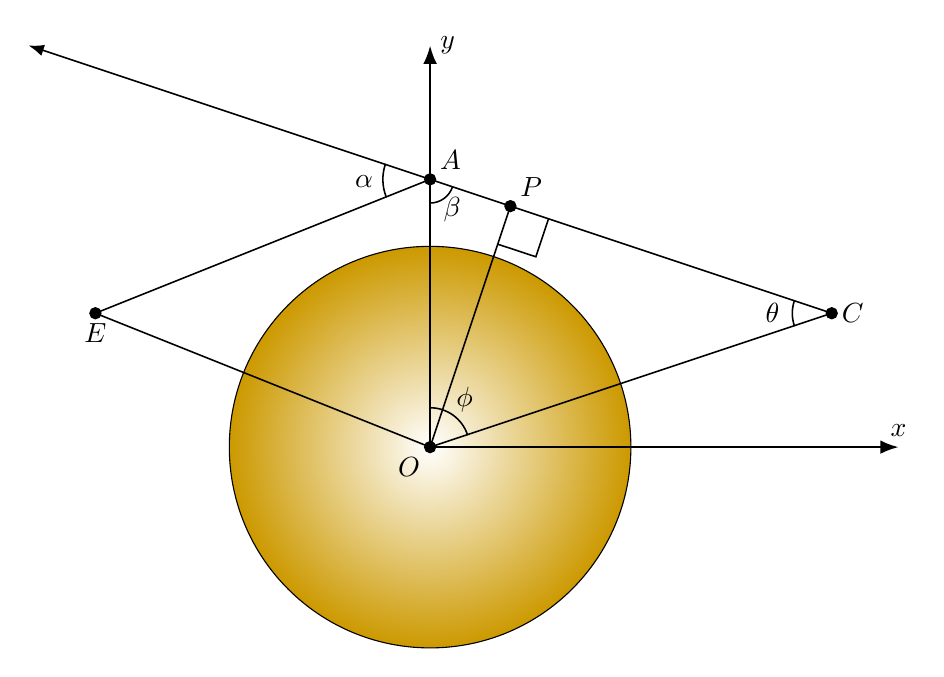
\begin{tikzpicture}[%
        > = Latex,
        line width = 0.2mm,
        line cap = round,
        scale = 1.7
    ]

        % Start a group to locally define variable for color.
        \begingroup

            % Color for the central ball.
            \newcommand{\bcolor}{orange!80!green}

            % coordinates
            \coordinate (O) at (0.0, 0.0); % Origin.
            \coordinate (E) at (-2.5, 1.0); % Earth.
            \coordinate (C) at (3.0, 1.0); % Cassini spacecraft.
            \coordinate (A) at (0.0, 2.0); % Point along axis of symmetry.
            \coordinate (P) at (0.6, 1.8); % Perpendicular on line CA.
            \coordinate (S) at (-3.0, 3.0); % Point in space along line CA.

            % Central circle.
            \draw[%
                inner color = white,
                outer color = \bcolor,
                thin
            ] (O) circle (1.5);

            % Axes.
            \begin{scope}[thick]
                \draw[->] (O) to (0.0, 3.0) node [right] {$y$};
                \draw[->] (O) to (3.5, 0.0) node [above] {$x$};
            \end{scope}

            % Various labels.
            \node at (O) [below left] {$O$};
            \node at (E) [below] {$E$};
            \node at (C) [right] {$C$};
            \node at (A) [above right] {$A$};
            \node at (P) [above right] {$P$};

            % Draw dots to mark various points.
            \draw[fill = black] (O) circle (0.4mm);
            \draw[fill = black] (E) circle (0.4mm);
            \draw[fill = black] (C) circle (0.4mm);
            \draw[fill = black] (A) circle (0.4mm);
            \draw[fill = black] (P) circle (0.4mm);

            % Draw lines connecting various points.
            \draw (O) to (P);
            \draw (O) to (E);
            \draw (O) to (C);
            \draw (A) to (E);

            % Draw a vector in the direction of the outgoing signal.
            \draw[->] (C) to (S);

            % Draw various angles.
            \pic[%
                "$\alpha$",
                angle eccentricity = 1.4,
                angle radius = 0.6cm,
                -,
                draw = black
            ] {angle = S--A--E};

            \pic[%
                "$\beta$",
                angle eccentricity = 1.6,
                angle radius = 0.3cm,
                -,
                draw = black
            ] {angle = O--A--C};

            \pic[%
                "$\theta$",
                angle eccentricity = 1.5,
                angle radius = 0.5cm,
                -,
                draw = black
            ] {angle = A--C--O};

            \pic[%
                "$\phi$",
                angle eccentricity = 1.5,
                angle radius = 0.5cm,
                -,
                draw = black
            ] {angle = C--O--A};

            % Draw square indicating right angle.
            \coordinate (tempa) at ($(P)!0.3cm!(O)$);
            \coordinate (tempb) at ($(P)!0.3cm!(C)$);
            \coordinate (tempc) at ($(tempa)!0.5!(tempb)$);
            \draw (tempa) to ($(P)!2!(tempc)$) to (tempb);
        \endgroup
    \end{tikzpicture}
\end{document}
